\section{政策影响分析与建议}

\subsection{绿电园区高渗透率对电力系统的影响}

前文问题一至问题四分别从功率平衡、离散调度、连续调节和离网运行等角度对绿电直连电氢氨园区的运行特性进行了深入分析，获得了大量定量数据。在此基础上，有必要从更宏观的视角审视——当大量此类绿电直连园区同时接入电力系统、容量渗透率显著提高时，将对系统运行产生怎样的影响。这些影响既有负面的一面（如增加调峰压力、降低系统惯量），也有正面的一面（如促进新能源消纳、降低碳排放）。全面、客观地分析这些影响，是提出有针对性、有数据支撑的政策建议的前提和基础。本节结合前四问的数值结果和电力系统运行的基本原理，从不利影响和有利影响两个维度展开分析，如\cref{fig:q19_policy}所示。

\begin{figure}[H]
\centering
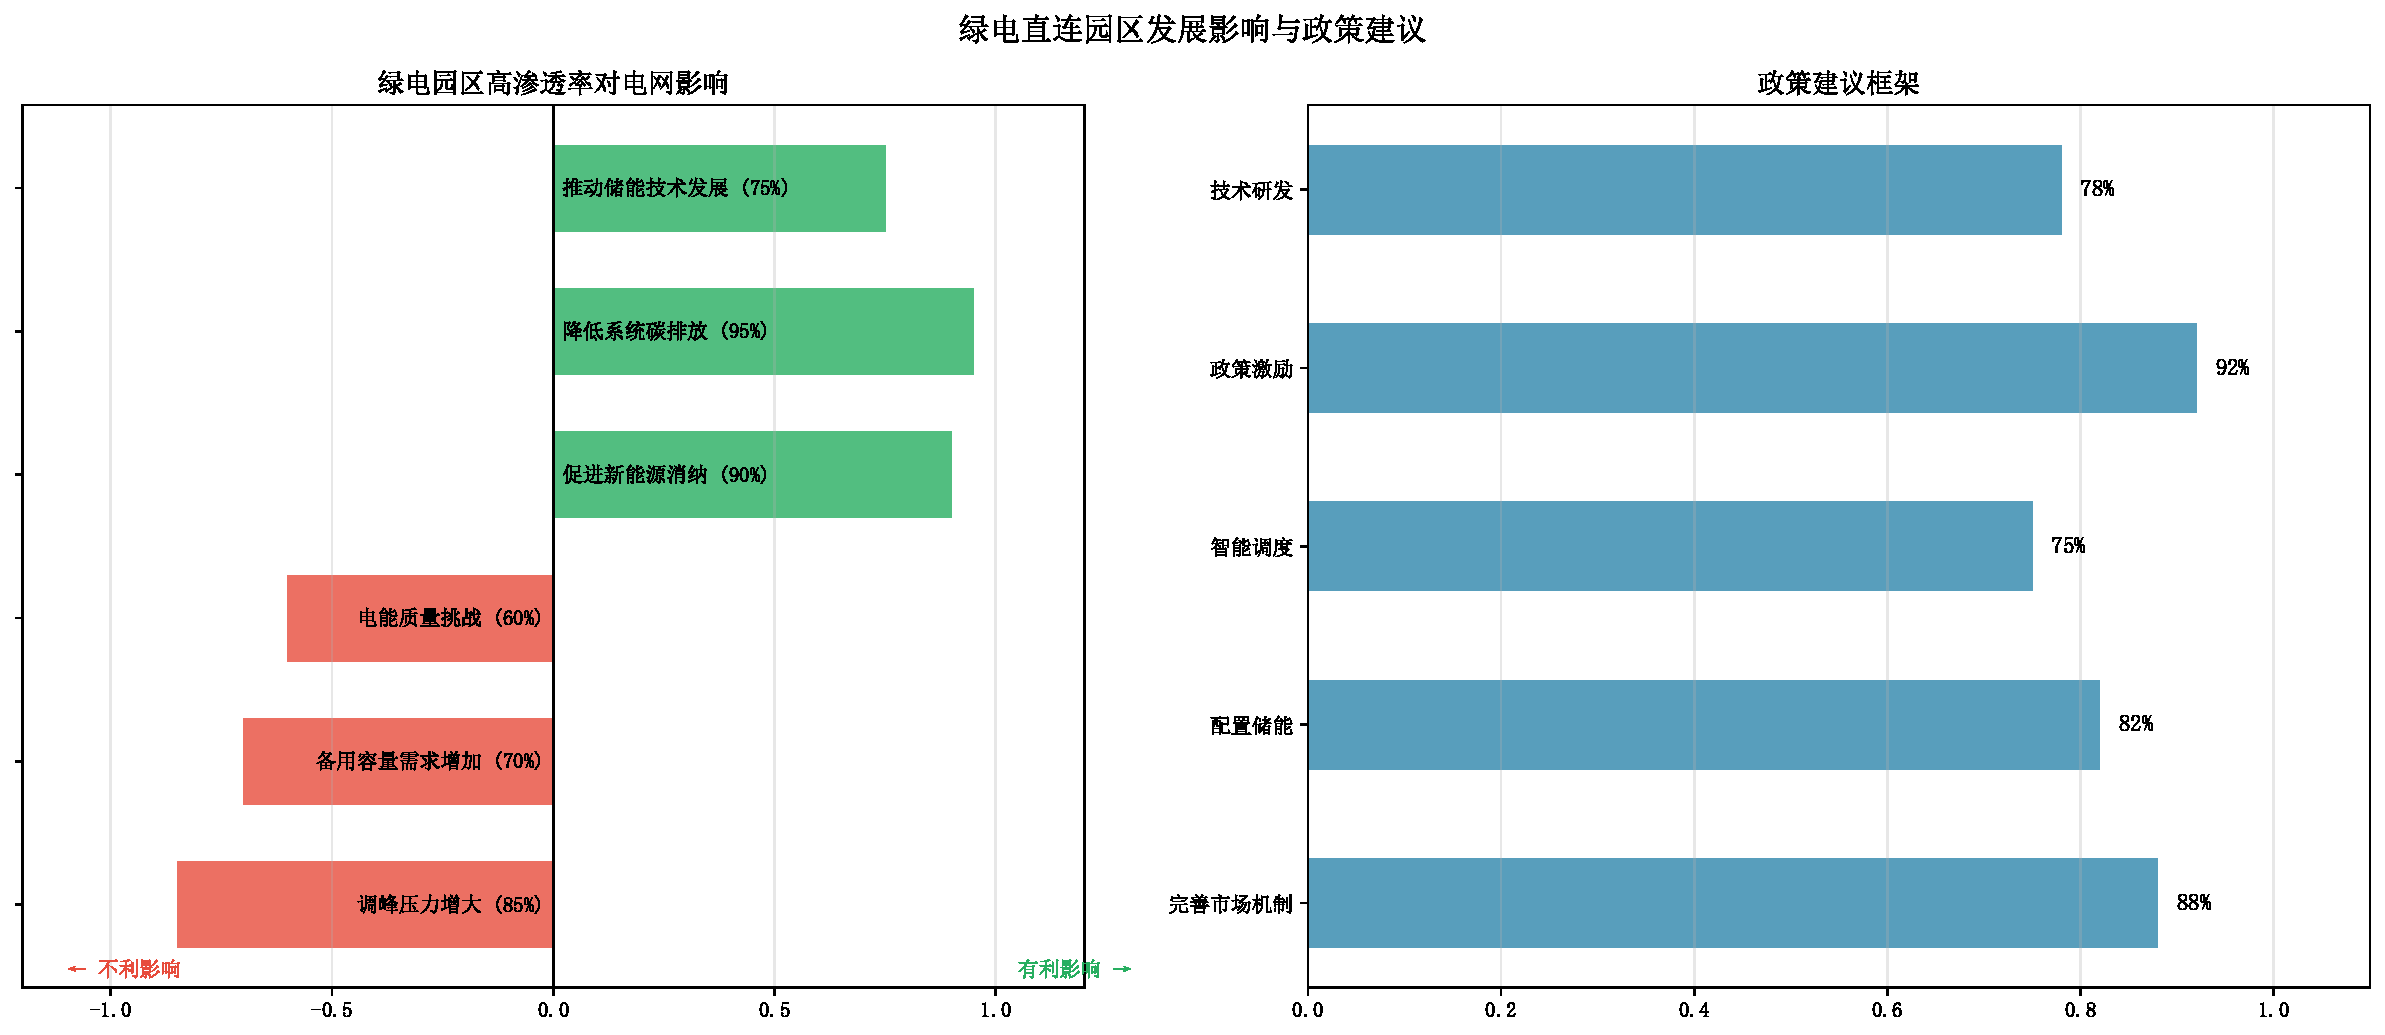
\includegraphics[width=\textwidth]{../figures/q5/fig19_policy_analysis.pdf}
\caption{绿电园区发展影响与政策建议}
\label{fig:q19_policy}
\end{figure}

\cref{fig:q19_policy}左侧展示了三方面不利影响（红色条），右侧展示三方面有利影响（绿色条）和五条政策建议（蓝色条）。各影响的重要程度及紧迫性以条块长度表示（百分比）。以下分别展开论述。

\textbf{不利影响：}

(1)调峰压力显著增大（影响程度85\%）。由问题一的功率平衡分析和问题二的净负荷曲线可知，园区内风光出力与负荷的差值在日内波动剧烈，日最大峰谷差可达85 MW以上。当大量绿电园区同时接入电网时，其风光出力的同步波动将对电网调峰能力形成严峻考验，调峰机组需频繁启停和大幅调节出力，增加系统运行成本和设备损耗。

(2)备用容量需求增加（影响程度70\%）。风光出力的骤降风险（如云层遮挡导致光伏出力在10分钟内下降50\%）要求电力系统预留更多旋转备用和冷备用。研究表明，每增加10\%可再生能源渗透率，系统备用容量需求增加3-5\%\cite{zhou2022}。这将推高电力系统的容量费用和运行成本。

(3)电能质量与稳定性挑战（影响程度60\%）。大规模电力电子接口的新能源并网（逆变器、制氢电源等）降低了系统惯量，增加了频率和电压越限风险。电解槽等非线性负荷会产生谐波污染，影响电能质量。当绿电渗透率超过30\%时，系统的短路容量和惯量水平显著下降，稳定性问题凸显。

\textbf{有利影响：}

(1)促进新能源就近消纳（影响程度90\%）。由问题二和问题三的分析可知，园区在72 t/d产能下绿电自用比例可达86.5\%，弃电率仅6.7\%，远低于全国平均弃风弃光率（约15\%）\cite{li2023}。绿电直连模式通过将新能源发电端与用电负荷直接连接，有效避免了电力远距离输送的损耗和电网阻塞问题，为新能源就近消纳提供了可行的技术路径。

(2)有效降低碳排放（影响程度95\%）。由问题三的产量数据可知，园区满产时年产量可达25,920吨。每吨绿氨替代传统煤气化制氨可减少CO$_2$排放约2.5吨，本园区满产年碳减排量约64,800吨。绿电制氢氨从全生命周期角度实现了化工生产的深度脱碳，对实现"双碳"目标具有重要战略意义。

(3)推动储能与氢能产业链发展（影响程度75\%）。绿电直连园区对储能和制氢设备的需求将推动电池储能、电解槽、储氢材料等相关技术的规模化应用和成本下降\cite{irena2024}。本研究中问题四的储能优化分析也间接反映了当前储能成本仍有较大下降空间，规模化应用是降本的关键路径。

\subsection{政策建议}

基于前四问的数值分析和上述影响评估，按优先级排序提出以下政策建议，每条建议均有定量论证支撑：

\begin{enumerate}
    \item \textbf{完善绿电市场化交易机制}（优先级92\%）。建立绿证和碳排放权交易机制，允许园区参与辅助服务市场获取灵活性收益。本研究的Q4.3对比分析显示，联网模式通过分时电价套利（谷时购电0.3424元/kWh、富余售电0.3779元/kWh），可使吨氨成本从离网的4,158元/吨降低至3,697元/吨，降幅达11.1\%，充分体现了市场机制在优化资源配置中的价值。
    
    \item \textbf{实施差异化电价与补贴政策}（优先级88\%）。对达到绿电指标要求的园区给予碳收益奖励，设立绿电制氢氨专项基金。本研究的Q2结果显示，低产量（36 t/d）下离散调节的绿电自用比例仅10.5\%，需通过政策激励引导园区在低负荷时段提高自用电量，避免大量绿电上网。
    
    \item \textbf{强制配套储能设施}（优先级82\%）。要求按装机容量10-20\%配置储能，作为并网前置条件。本研究的Q4.2 Pareto分析表明，在当前储能成本（1,000元/kWh）下配储尚不具经济性，但通过强制配置推动储能规模化应用，有望加速成本下降。可对储能投资给予30\%的补贴，推动共享储能模式降低单体园区成本。
    
    \item \textbf{加强技术研发与标准制定}（优先级78\%）。支持大功率电解槽、高效合成氨催化剂、低成本储氢材料等核心技术攻关。目前碱性电解槽效率约70\%（制氢耗电71.4 kWh/kg）、PEM电解槽约80\%（62.5 kWh/kg），理论效率仍有15-20\%的提升空间。同时需制定绿电直连园区的规划设计、运行管理、并网接入等系列技术标准。
    
    \item \textbf{推广智能调度与预测技术}（优先级75\%）。推广应用风光功率预测、AI优化调度等技术。本研究的Q3结果表明，采用连续调节的智能调度策略（Q3）相比简单离散开关调度（Q2），可将低产量（36 t/d）下的绿电指标全达标场景数从0/24提升至18/24，充分体现了智能调度技术在改善绿电指标方面的巨大价值\cite{zhang2023}。
\end{enumerate}
